
\documentclass[10pt]{beamer}

\usepackage{beamerthemesplit}
\usepackage{amsmath}
\usepackage{amssymb,mathpartir}
\usepackage{amsthm}
\usepackage{graphicx}
%\usepackage[latin1]{inputenc}



\useoutertheme{infolines}

\title{The Boyer-Moore Family of Automated Theorem Provers}

\author{Dionna Glaze}

\date{September 28th, 2009}

\definecolor{blue}{rgb}{0,0,1.0}
\newcommand{\blue}[1]{{\color{blue}#1}}
\definecolor{green}{rgb}{0,1.0,0}
\newcommand{\green}[1]{{\color{green}#1}}
\definecolor{red}{rgb}{1.0,0,0}
\newcommand{\red}[1]{{\color{red}#1}}
\definecolor{grey}{rgb}{0.6,0.6,0.6}
\newcommand{\grey}[1]{{\color{grey}#1}}

\AtBeginSection[]
{
\begin{frame}<beamer>
  \frametitle{Outline}
  \tableofcontents[currentsection]
\end{frame}
}


    \begin{document}


\frame{\titlepage}

\frame{
\frametitle{Outline}
\tableofcontents
}

\section{Introduction}

\frame{
\frametitle{Hisorical Motivation}
``Instead of trying out computer programs on test cases until they are debugged, one should prove that they have the desired properties.'' \\
John McCarthy [A Basis For A Mathematical Theory of Computation]
}
%%%%%%%%%%%%%%%%%%%%%%%%%%%%%%%%%%%%%%%%%%%%%%%%%%%%%
\frame{
\frametitle{Boyer, Moore, and the Actualization}
\begin{itemize}
  \item Pure Lisp Theorem Prover (Associativity of Append)
  \item NQTHM (G\"odel's Second Incompleteness Theorem)
  \item ACL2 (Correctness of K5)
\end{itemize}
}
%%%%%%%%%%%%%%%%%%%%%%%%%%%%%%%%%%%%%%%%%%%%%%%%%%%%%
\frame{
\frametitle{The Boyer-Moore Approach}
In \textit{A Computational Logic}, Boyer and Moore described a way to automatically deduce good induction schemes to prove the correctness of recursively defined functions. \\
\begin{itemize}
  \item Use structure to induct.
  \item Simplify terms through rewriting.
  \item Use total functions.
  \item No higher order functions.
  \item Take risks.
\end{itemize}
}
%%%%%%%%%%%%%%%%%%%%%%%%%%%%%%%%%%%%%%%%%%%%%%%%%%%%%
\section{Computational Logic}

%%%%%%%%%%%%%%%%%%%%%%%%%%%%%%%%%%%%%%%%%%%%%%%%%%%%%
\frame{
\frametitle{What is Proof?}
\begin{itemize}
  \item An appeal is a list of $(method\ conclusion\ subproofs\
    extras)$
  \item $method$ is a rule of inference you trust as validity
    preserving. 
  \item \texttt{t} $\Rightarrow$ axioms, theorems,
    propositional schema, functional equality, beta reduction and base
    evaluation.
  \item Other methods rely on previously proven statements and/or
    other elements such as a substitution function, $\sigma$.
  \item A proof is an appeal or list of appeals.
\end{itemize}
}
%%%%%%%%%%%%%%%%%%%%%%%%%%%%%%%%%%%%%%%%%%%%%%%%%%%%%
\frame{
\frametitle{Axiomatized Semantics}
ACL2 has hundreds of axioms regarding certain Lisp primitive functions
and the behavior of complex rationals. \\
\begin{align*}
\text{\texttt{(or }} & \text{\texttt{(not (equal x 'nil))}} \\
               & \text{\texttt{(equal (if x y z) z))}} 
\end{align*}
\begin{align*}
\text{\texttt{(equal (car (cons x y)) x)}} 
\end{align*}
\begin{align*}
\text{\texttt{(or }} & \text{\texttt{(equal (natp a) 'nil)}} \\
                     & \text{\texttt{(equal (< a b) 't)}} \\
                     & \text{\texttt{(equal (< b a) 't)}} \\
                     & \text{\texttt{(equal a b))}}
\end{align*}
}
%%%%%%%%%%%%%%%%%%%%%%%%%%%%%%%%%%%%%%%%%%%%%%%%%%%%%
\frame{
\frametitle{Rules of inference, some axioms}
\begin{columns}[2]
  \column{.4\textwidth}
  \renewcommand{\arraystretch}{2}
  \begin{tabular}{p{2.2cm} l}
    Propositional Schema & \scriptsize{$\inferrule{ }{\neg A \vee A}
      $}\\
    Contraction & \scriptsize{$\inferrule{A \vee A}{A}$} \\
    Expansion & \scriptsize{$\inferrule{A}{B \vee A}$} \\
    Associativity & \scriptsize{$\inferrule{A \vee (B \vee C)}{(A \vee B) \vee C}$}
    \\
    Cut & \scriptsize{$\inferrule{A \vee B \\ \neg A \vee C}{B \vee C}$} \\
    Instantiation & \scriptsize{$\inferrule{A}{A/\sigma}$} \\
    Induction & ...
  \end{tabular}

  \column{.55\textwidth}
    Reflexivity Axiom \\
      \quad {\scriptsize $x = x$} \\
    \hspace*{\fill} \\
    Equality Axiom \\
      \quad {\scriptsize $x_1 = y_1 \rightarrow x_2 = y_2 \rightarrow x_1
    = x_2 \rightarrow y_1 = y_2$} \\
    \hspace*{\fill} \\
    Referential Transparency \\
      \quad {\scriptsize $x_1 = y_1 \rightarrow ... \rightarrow
    x_n = y_n \rightarrow f(x_1,...,x_n) = f(y_1, ..., y_n)$} \\
    \hspace*{\fill} \\
    Beta Reduction \\
      \quad {\scriptsize $((\lambda x_1 ... x_n . \beta) t_1 ... t_n) =
    \beta / \left[x_1 \leftarrow t_1, ..., x_n \leftarrow t_n
    \right]$} \\
    \hspace*{\fill} \\
    Base Evaluation \\
      \quad {\scriptsize e.g. $1 + 2 = 3$} \\
    \hspace*{\fill} \\
    Lisp Axioms \\ 
      \quad {\scriptsize e.g. \texttt{(consp (cons x y)) = t}}
\end{columns}
}
%%%%%%%%%%%%%%%%%%%%%%%%%%%%%%%%%%%%%%%%%%%%%%%%%%%%%
\frame{
\frametitle{Extending the Logic}
In ACL2 and Milawa, extending the logic with new theorems or
definitions comes in the form of
\textit{events}. \\
An event adds to the history of sound extensions to the logic, and can
be in one of three forms:
\begin{itemize}
  \item Theorem
  \item Recursive function definition
  \item Skolem (witnessing) function definition
\end{itemize}
Each of which has the obligation of proving its \textit{admissibility}.
}
%%%%%%%%%%%%%%%%%%%%%%%%%%%%%%%%%%%%%%%%%%%%%%%%%%%%%
\frame{
\frametitle{Function Definition Events}
A recursive function definition $(\text{\texttt{equal}}\ (f\ x_1\
...\ x_n)\ \beta)$ (with its measure $m$) is \textit{admissible} to a
history $h$ if and only if the following statements are true:
\begin{itemize}
  \item The function name is not already used.
  \item The $FREEVARS(\beta)$ and $FREEVARS(m)$ are subsets of $\{x_1\
    ...\ x_n\}$.
  \item $\beta$ is well formed with respect to the history (no
  undefined function calls, etc).
  \item The following formulas (\textit{termination obligations}) are provable from $h$:
  \begin{itemize}
    \item Ordinal obligation: \\
      \quad \texttt{(equal (ordp m) t)}
    \item Progress obligation: \\
      \quad For each recursive call $(f\ a_1\ ...\ a_n)$, \\
      \quad \texttt{(equal (ord< }$m/\left[x_1 \leftarrow a_1, ...,
        x_n \leftarrow a_n\right]\ m$\texttt{) t)}
  \end{itemize}
\end{itemize}
}
%%%%%%%%%%%%%%%%%%%%%%%%%%%%%%%%%%%%%%%%%%%%%%%%%%%%%
\frame{
\frametitle{Skolem Functions}
Banach-Tarski Paradox be damned, I like the axiom of choice. \\
\pause
\begin{itemize}
\item A Skolem function is a non-executable function with a bound variable
$\nu$, free variables $x_1\ ...\ x_n$ (disjoint from $\nu$) with body
$\beta$.
\pause
\item The effect of defining a Skolem function is a new axiom, 
  \begin{align*}
    \text{\texttt{(or }} & \text{\texttt{(equal }} \beta
    \text{\texttt{ nil)}}  \\
                         & \text{\texttt{(not (equal ((}} 
                         \text{\texttt{lambda (}} \nu\ x_1\ ...\ x_n
                         \text{\texttt{) }} \beta \text{\texttt{)}} \\
                         & \qquad \qquad \qquad \qquad \qquad \text{\texttt{(}} f\ x_1\ ...\ x_n
                         \text{\texttt{) }} x_1\ ...\ x_n
                         \text{\texttt{)}}\\
                         & \qquad \qquad \qquad \text{\texttt{nil)))}}
  \end{align*}
\pause
\item To be abmissible, the name of $f$ must be new,
  $FREEVARS(\beta)$ must be a subset of $\{\nu, x_1, ..., x_n\}$, and
  $beta$ is well formed with respect to the history.
\pause
\item Great for making canonical prepresentations of equivalence
  classes and reasoning about quantification.
\end{itemize}
}
%%%%%%%%%%%%%%%%%%%%%%%%%%%%%%%%%%%%%%%%%%%%%%%%%%%%%

\section{Theorem Proving}

\frame{
\frametitle{Rewriting}
The key to proving theorems is by rewriting equivalent statements (or
instantiating more general statements) into a form that give you the
conclusion you are looking for.\\
\pause
What do I mean by that? Well...\\
\pause
Example:\\ 
\begin{align*}
\text{\texttt{(implies (and }} & \text{\texttt{(true-listp x)}} \\
                               & \text{\texttt{(true-listp y)}} \\
                               & \text{\texttt{(true-listp z))}} \\
                               & \text{\texttt{(equal (append x
                                   (append y z))}} \\
                               & \qquad \qquad \text{\texttt{(append (append
                                   x y) z))}}
\end{align*}
}
%%%%%%%%%%%%%%%%%%%%%%%%%%%%%%%%%%%%%%%%%%%%%%%%%%%%%
\frame{
\frametitle{ACL2: Proof Checker $\rightarrow$ Theorem Prover}
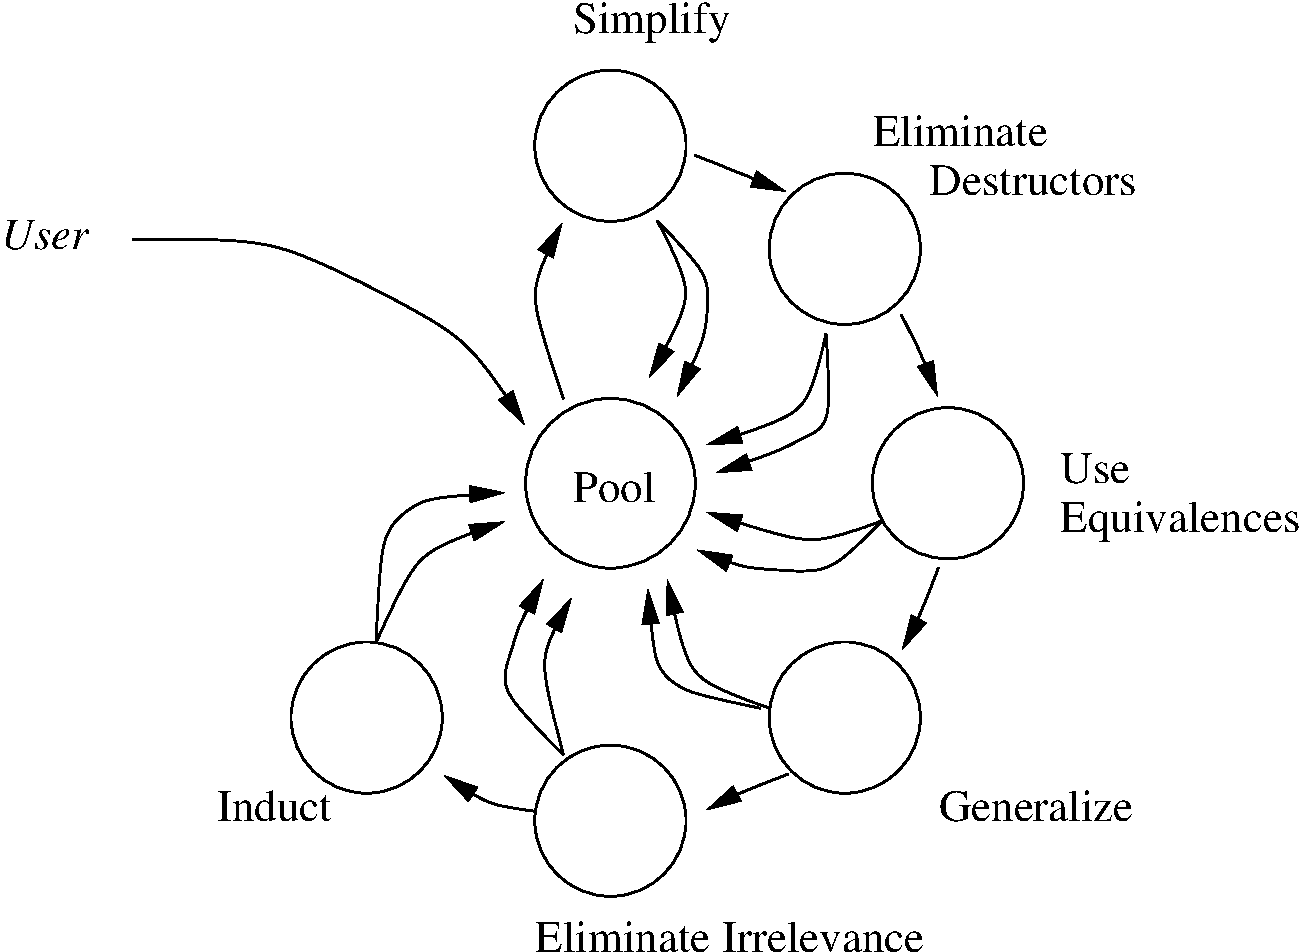
\includegraphics[scale=0.3]{waterfall.pdf} \\
\pause
Rewriting (simplification) is validity preserving, but in difficult
theorems, we want to talk more abstractly without having to build the
trivial ground theory ourselves. This is where the Boyer-Moore
``waterfall'' and it's increasingly risky heuristics step in.
}
%%%%%%%%%%%%%%%%%%%%%%%%%%%%%%%%%%%%%%%%%%%%%%%%%%%%%
\frame{
\frametitle{Destructor Elimination}
\begin{itemize}
\item The first step in generalizing statements is to remove ``destructors''
(observers), and replace them with their constructive counterparts.
\item This step tends to make arguments smaller and cleaner looking,
  e.g. \\
{\scriptsize
\begin{align*}
\text{\texttt{(implies }} & \text{\texttt{(and (true-listp x)}} \\ 
                          & \qquad \quad \text{\texttt{(equal (reverse
                              (reverse (cdr x))) (cdr x)))}} \\
                          & \text{\texttt{(equal (reverse (append
                              (reverse (cdr x)) (cons (car x) nil)))}}
                          \\ 
                          & \qquad \qquad \text{\texttt{x))}}
\end{align*}}
\pause
becomes \\
{\scriptsize
\begin{align*}
\text{\texttt{(implies }} & \text{\texttt{(and (true-listp b)}} \\ 
                          & \qquad \quad \text{\texttt{(equal (reverse
                              (reverse b)) b))}} \\
                          & \text{\texttt{(equal (reverse (append
                              (reverse b) (cons a nil)))}} \\
                          & \qquad \qquad \text{\texttt{(cons a b)))}}
\end{align*}}
\end{itemize}
}
%%%%%%%%%%%%%%%%%%%%%%%%%%%%%%%%%%%%%%%%%%%%%%%%%%%%%
\frame{
\frametitle{Using Equivalences}
Also called, ``cross-fertilization''.
\begin{itemize}
  \item It is often useful to use equality hypotheses to replace equal
    terms in the conjecture's conclusion.
  \item In some cases we can use this cross fertilization to eliminate
    the equality hypothesis entirely and create a more general
    conjecture, e.g. in proving the commutativity of plus in Peano
    arithmetic.
\end{itemize}
\pause
\begin{align*}
\text{\texttt{(implies }} & \text{\texttt{(and (not (zp y))}} \\
                          & \qquad \text{\texttt{(equal (plus x (sub1
                              y))}} \\
                          & \qquad \qquad \text{\texttt{(plus (sub1 y)
                              x)))}} \\
                          & \text{\texttt{(equal (plus x y) (plus y
                              x)))}}
\end{align*}
\pause
after destructor elimination becomes
\begin{align*}
\text{\texttt{(implies }} & \text{\texttt{(equal (plus x y) (plus y
    x))}} \\
                          & \text{\texttt{(equal (plus x (add1 y))}}
                          \\
                          & \qquad \text{\texttt{(add1 (plus y x))))}}
\end{align*}                          
}
%%%%%%%%%%%%%%%%%%%%%%%%%%%%%%%%%%%%%%%%%%%%%%%%%%%%%
\frame{
\frametitle{Cross-fertilization example (continued)}
After cross-fertilization we have
\begin{align*}
\text{\texttt{(equal (plus x (add1 y)) (add1 (plus x y)))}}
\end{align*}
\pause
Which we can prove by induction on \texttt{x}. Our induction step is
\begin{align*}
\text{\texttt{(implies }} & \text{\texttt{(equal (plus x (add1 y))}}
\\
                          & \qquad \text{\texttt{(add1 (plus x y)))}}
                          \\
                          & \text{\texttt{(equal (plus (add1 x) (add1
                              y))}} \\
                          & \qquad \text{\texttt{(add1 (plus (add1 x) y))))}}
\end{align*}
\pause
We cross-fertilize again to get
\begin{align*}
\text{\texttt{(equal }} & \text{\texttt{(add1 (plus x (add1 y)))}} \\
                        & \text{\texttt{(add1 (add1 (plus x y))))}}
\end{align*}
\pause
This simplifies to our induction hypothesis, thus it is proven.
}
%%%%%%%%%%%%%%%%%%%%%%%%%%%%%%%%%%%%%%%%%%%%%%%%%%%%%
\frame{
\frametitle{Generalization}
\begin{itemize}
  \item Many times when we try to prove things about our functions, the same
thing is true for any \texttt{x}.
\pause
  \item However, it's not too difficult to think of a case where this
    is not true.
\pause
  \item Thus generalization lemmas are allowed to be considered for
    assigning type information to a generalized statement.
\pause
  \item If the type information is too general, say it is a union
    type, it is typically disadvantageous to use that information.
\pause
  \item One must also make sure not to go overboard with
    generalization, lest he inadvertantly add complexity to the proof.
\end{itemize}
}
%%%%%%%%%%%%%%%%%%%%%%%%%%%%%%%%%%%%%%%%%%%%%%%%%%%%%
\frame{
\frametitle{Eliminating Irrelevance}
\begin{itemize}
  \item Sometimes the user or the generalization process will introduce more
hypotheses than are necessary to prove a conjecture. 
\pause
  \item It is advantageous to remove irrelevant hypotheses so we can
    generate a more easily proven induction scheme.
\pause
  \item By partitioning hypotheses by shared variables, we can use
    some heuristics to guess which clauses are probably falsifiable
    and eliminate them.
\pause
  \item This always results in a more general statement, so in the
    case the heuristics fail and remove an important hypothesis, the
    original conjecture is still a theorem if the new statement is a
    theorem.
\end{itemize}
}
%%%%%%%%%%%%%%%%%%%%%%%%%%%%%%%%%%%%%%%%%%%%%%%%%%%%%
\frame{
\frametitle{Induction and Recursion}
Why use induction at the end if it's so well connected to the
recursive definition of a function?
\begin{itemize}
  \item  Induction introduces new subgoals rather than dispelling old
    ones.
\pause
  \item Many statements are not amenable to proof by induction.
\pause
  \item If a rewrite rule can be used before attacking the entire
    structure of a definition to prove a conjecture, we should do
    that.
\pause
  \item Induction schemes explode on very specific statements, so it
    is best to induct on the most general possible statement of the
    conjecture.
\end{itemize}
}
%%%%%%%%%%%%%%%%%%%%%%%%%%%%%%%%%%%%%%%%%%%%%%%%%%%%%
\section{Reading}

\frame{
\frametitle{References}
\begin{itemize}
\item A Self-Verifying Theorem Prover, Ph.D. Thesis at UT Austin by Jared Davis.
\item A Computational Logic, by Bob Boyer and J Moore.
\item A Basis For A Mathematical Theory of Computation, by John McCarthy.
\end{itemize}
And thanks to Jared Davis for his contribution to the preparation of
this talk.
}
%%%%%%%%%%%%%%%%%%%%%%%%%%%%%%%%%%%%%%%%%%%%%%%%%%%%%
\frame{
\frametitle{Questions}
Speak now...
}

\end{document}

